\chapter{Bayesian nonparametric}

\section{Definition} \label{BNP_def}
A Bayesian nonparametric model is a model that (i) constitutes a Bayesian model on an infinite-dimensional parameter space and (ii) can be evaluated on a finite sample in a manner that uses only a finite subset of the available parameters to explain the sample.
The parameter space in (i) typically consists of functions or of measures, while (ii) is usually achieved by marginalizing out surplus dimensions over the prior. Random functions and measures, and more generally probability distributions on infinite-dimensional random objects, are called stochastic processes.


\section{Motivation}
% Model selection
Most scientists address the model selection problem by first fitting several models, with different numbers of clusters or factors, and then selecting one using model comparison metrics \cite{Claeskens:1251912}. Model selection metrics usually include two terms. The first term measures how well the model fits the data. The second term, a complexity penalty, favors simpler models (i.e., ones with fewer components or factors).

\gls{BNP} models provide a different approach to this problem. Rather than comparing models that vary in complexity, the \gls{BNP} approach is to fit a single model that can adapt its complexity to the data. \gls{BNP} models allow the complexity to grow as more data are observed, such as when using a model to perform prediction. This is an attractive property for many settings.

%Popular examples of Bayesian nonparametric models include Gaussian process regression, in which the correlation structure is refined with growing sample size, and Dirichlet process mixture models for clustering, which adapt the number of clusters to the complexity of the data.

\subsection{Exchangeability}

The underlying assumption of all Bayesian methods is that the parameter specifying the observation model is a random variable. 
However, there is a very general type of so-called \textit{exchangeable} observations for which the existence of such a random variable is a mathematical consequence of the data's properties. This is an important notion since all models we will be considering in Chapter \ref{BNP_PPL} are assuming exchangeability.

Formally, a sequence of variables $X_1,\dots,X_n$ over the same probability space $(\mathbb{X},\Omega)$ is \textit{exchangeable} if their joint distribution is invariant to permuting the variables. That is, if for any permutation $\sigma$ of $\{1,\dots,n\}$, then
$$ \mathbb{P}(X_1=x_1,\dots,X_n=x_n) = \mathbb{P}(X_1=x_{\sigma(1)},\dots,X_n=x_{\sigma(n)}) $$

Exchangeability reflects the assumption that the variables do not depend on their indices although they may be dependent among themselves. This is typically a reasonable assumption in machine learning and statistical applications, even if the variables are not themselves iid, since it is a much weaker assumption.

If $\theta$ parametrizes the underlying distribution, and one assumes a prior distribution over $\theta$, then the resulting marginal distribution over $X_1,\dots,X_n$ with $\theta$ marginalized out will still be exchangeable. A fundamental result credited to de Finetti \cite{finetti31} states that the converse is also true. That is, if $X_1,\dots,X_n$ is exchangeable, then there is a random $\theta$ such that:
\begin{equation} \label{eq:deFineti}
P(X_1,\dots,X_n) = \int{P(\theta)\prod_{i=1}^n{P(X_i|\theta) d\theta}}
\end{equation}
In other words, the seemingly innocuous assumption of exchangeability automatically implies the existence of a hierarchical Bayesian model with $\theta$ being the random latent parameter.

In de Finetti’s Theorem it is important to stress that $\theta$ can be infinite dimensional (it is typically a random measure), thus the hierarchical Bayesian model \ref{eq:deFineti} is typically a nonparametric one. For example, the Blackwell-MacQueen urn scheme (related to the \gls{CRP}) is exchangeable thus implicitly defines a random measure, namely the \gls{DP}.

% Applications

\section{Examples}
Bayesian nonparametric models have recently been applied to a variety of machine learning problems, including regression, classification, clustering, latent variable modeling, sequential modeling, image segmentation, source separation and grammar induction.


\subsection{\acrlong{DP}} \label{DP}

The \acrfull{DP} is a distribution over distributions. It is parameterized by a concentration parameter $\alpha > 0$ and a base distribution $H_0$, which is a distribution over a space $\mathbb{X}$. A random variable drawn from a \gls{DP} is itself a distribution over $\mathbb{X}$. A random distribution $P$ drawn from a \gls{DP} is denoted $P \sim \text{DP}(\alpha, H_0)$.

The \gls{DP} was first developed in \cite{ferguson73}, who showed its existence by appealing to its finite dimensional distributions. Consider a measurable partition of $\mathbb{X}$, $\{A_1,\dots,A_K\}$ If $P \sim \text{DP}(\alpha, H_0)$ then every measurable partition of $\mathbb{X}$ is Dirichlet-distributed,
$$(P(A_1), \dots , P(A_K)) \sim \text{Dir}(\alpha H_0(A_1), \dots , \alpha H_0(A_K)).$$

This means that if we draw a random distribution from the \gls{DP} and add up the probability mass in a region $A \in \mathbb{X}$, then there will on average be $H_0(A)$ mass in that region. The concentration parameter plays the role of an inverse variance; for higher values of $\alpha$, the random probability mass $P(A)$ will concentrate more tightly around $H_0(A)$.

\cite{ferguson73} proved two properties of the Dirichlet process. The first property is that random distributions drawn from the Dirichlet process are discrete. They place their probability mass on a countably infinite collection of points, called “atoms,”
\begin{equation} \label{eq:DP}
P = \sum_{k=1}^\infty{p_k \delta_{X_k^\star}}.
\end{equation}
where $p_k$ is the probability assigned to the $k$th atom and $X_k^\star$ is the location or value of that atom. Further, these atoms are drawn independently from the base distribution $H_0$.

The second property connects the Dirichlet process to the Chinese restaurant process. Consider a random distribution drawn from a DP followed by repeated draws from that random distribution,
\begin{gather}
P \sim \text{DP}(\alpha, H_0) \\
X_i \sim P \quad \forall i= \{1,\dots,n\} \label{eq:CRP}
\end{gather}

\cite{ferguson73} examined the joint distribution of $X_{1:n}$, which is obtained by marginalizing out the random distribution $P$,
\begin{equation}
p(X_1,\dots,X_n|\alpha,H_0) = \int{\left(\prod_{i=1}^n p(X_i|P) \right) d \mathbb{P}(P|\alpha,H_0)}
\end{equation}

He showed that, under this joint distribution, the $X_i$ will exhibit a \textit{clustering property}--they will share repeated values with positive probability. The structure of shared values defines a partition of the integers from $1$ to $n$, and the distribution of this partition is a Chinese restaurant process with parameter $\alpha$. Finally, he showed that the unique values of $X_i$ shared among the variables are independent draws from $H_0$.

\paragraph{The stick-breaking construction}
\cite{ferguson73} proved that the \gls{DP} exists via its finite dimensional distributions. \cite{sethuraman94} provided a more constructive definition based on the stick-breaking representation.

Consider a stick with unit length. We divide the stick into an infinite number of segments $\tilde{p}_k$ by the following process. First, choose a beta random variable $Z_1 \sim \text{beta}(1, \alpha)$ and break of $V_1$ of the stick. For each remaining segment, choose another beta distributed random variable, and break off that proportion of the remainder of the stick. This gives us an infinite collection of weights 
\begin{gather}
V_k \sim \text{beta}(1, \alpha) \\
\tilde{p}_k = V_k \prod_{j=1}^{k-1}(1-V_j) \quad k= 1,2,\dots \label{eq:SB_DP}
\end{gather}
Finally, we construct a random distribution using Equation \ref{eq:DP}, where we take an infinite number of draws from a base distribution $H_0$ and draw the weights as in Equation \ref{eq:SB_DP}. \cite{sethuraman94} showed that the distribution of this random distribution is a $DP(\alpha,H_0)$.
%This representation of the Dirichlet process, and its corresponding use in a Dirichlet process mixture, allows us to compute a variety of functions of posterior DPs (Gelfand and Kottas, 2002) and is the basis for the variational approach to approximate inference (Blei and Jordan, 2006).

\paragraph{\acrlong{CRP}}
The \gls{CRP} is a distribution over infinite partitions of the integers \cite{PitmanCRP,AldousCRP}.
The \gls{CRP} derives its name from the following metaphor. Imagine a restaurant with an infinite number of tables \footnote{The Chinese restaurant metaphor is due to Pitman and Dubins, who were inspired by the seemingly infinite seating capacity of Chinese restaurants in San Francisco.}, and imagine a sequence of customers entering the restaurant and sitting down. The first customer enters and sits at the first table. The second customer enters and sits at the first table with probability $\frac{1}{1+\alpha}$, and the second table with probability $\frac{\alpha}{1+\alpha}$, where $\alpha$ is a positive real. When the $n$th customer enters the restaurant, he sits at each of the occupied tables with probability proportional to the number of previous customers sitting there, and at the next unoccupied table with probability proportional to $\alpha$. At any point in this process, the assignment of customers to tables defines a random partition.

More formally, let $z_n$ be the table assignment of the $n$th customer. A draw from this distribution
\begin{equation*}
P(z_n = k | \mbz_{1:n-1})
\propto \begin{cases} \frac{m_k}{n-1+\alpha} \ \text{if} \ k \le K_+\ \text{(i.e., k is a previously occupied table)} \\ 
 \frac{\alpha}{n-1+\alpha} \ \text{otherwise} \ \text{(i.e., k is the next unoccupied table)} \end{cases}
\end{equation*}
where $m_k$ is the number of customers sitting at table $k$, and $K_+$ is the number of tables for which $m_k > 0$.

\paragraph{Dirichlet process mixtures}
A \gls{DP} mixture adds a third step to the model above: $Y_i \sim f(\cdot|X_i)$. Marginalizing out $P$ reveals that the \gls{DP} mixture is equivalent to a \gls{CRP} mixture. Moreover, the stick-breaking representation is a generative process enabling to lazily sample according to the associated \gls{DP}, in a \textit{size-biased} order. We will talk more about this size-biased of the \gls{DP} atoms in Proposition \ref{prop:perman} and its discussion.


\subsection{Nonlinear regression}
The aim of regression is to infer a continuous function from a training set consisting of input-output pairs $\{(t_i , x_i )\}_{i=1}^n$. Parametric approaches parametrize the function using a finite number of parameters and attempt to infer these parameters from data. The prototypical Bayesian nonparametric approach to this problem is to define a prior distribution over continuous functions directly by means of a \gls{GP}. As explained in \cite{Rasmussen:2005:GPM:1162254}, a \gls{GP} is a distribution on an infinite collection of random variables $X_t$, such that the joint distribution of each finite subset $X_{t_1},\dots, X_{t_n}$ is a multivariate Gaussian. A value $x_t$ taken by the variable $X_t$ can be regarded as the value of a continuous function $f$ at $t$, that is, $f(t) = x_t$. Given the training set, the Gaussian process posterior is again a distribution on functions, conditional on these functions taking values $f(t_1)=x_1,\dots,f(t_n)=x_n$.

\subsection{Latent feature models}
Latent feature models represent a set of objects in terms of a set of latent features, each of which represents an independent degree of variation exhibited by the data. Such a representation of data is sometimes referred to as a distributed representation. %#In analogy to nonparametric mixture models with an unknown number of clusters, a Bayesian nonparametric approach to latent feature modeling allows for an unknown number of latent features.
A Bayesian nonparametric approach to latent feature modeling allows for an unknown number of latent features.
The stochastic processes involved here are known as the \gls{IBP} and the \gls{BP}. Draws from \glspl{BP} are random discrete measures, where each of an infinite number of atoms has a mass in $(0,1)$ but the masses of atoms need not sum to $1$. Each atom corresponds to a feature, with the mass corresponding to the probability that the feature is present for an object. We can visualize the occurrences of features among objects using a binary matrix, where the $(i,k)$ entry is $1$ if object $i$ has feature $k$ and $0$ otherwise. The distribution over binary matrices induced by the \gls{BP} is called the \gls{IBP}.

\subsection{Hidden Markov models}
\glspl{HMM} are popular models for sequential or temporal data, where each time step is associate with a state, with state transitions dependent on the previous state. An infinite \gls{HMM} is a Bayesian nonparametric approach to \glspl{HMM}, where the number of states is unbounded and allowed to grow with the sequence length. It is defined using one \gls{DP} prior for the transition probabilities going out from each state. To ensure that the set of states reachable from each outgoing state is the same, the base distributions of the \glspl{DP} are shared and given a \gls{DP} prior recursively. The construction is called a \gls{HDP}.

\subsection{Density estimation}
A nonparametric Bayesian approach to density estimation requires a prior on densities or distributions. However, the \gls{DP} is not useful in this context, since it generates discrete distributions. A useful density estimator should smooth the empirical density (such as a Parzen window estimator), which requires a prior that can generate smooth distributions. Priors applicable in density estimation problems include \gls{DP} mixture models and Pólya trees.

%Since the mixing distribution in the \gls{DP} mixture is random, the induced density $p(x)$ is random thus the \gls{DP} mixture can be used as a prior over densities. Despite the fact that these are now primarily used in machine learning as clustering models, they were in fact originally proposed for density estimation.

%Pólya Trees are priors on probability distributions that can generate both discrete and piecewise continuous distributions, depending on the choice of parameters. Pólya trees are defined by a recursive infinitely deep binary subdivision of the domain of the generated random measure. Each subdivision is associated with a beta random variable which describes the relative amount of mass on each side of the subdivision. The \gls{DP} is a special case of a Pólya tree corresponding to a particular parametrization. For other parametrizations the resulting random distribution can be smooth so is suitable for density estimation.





\section{Mixture models}
\subsection{Finite dimensional}
Mixture models provide a statistical framework for modeling data where each observation is assumed to have arisen from one of $k$ groups, with $k$ possibly unknown, and each group being suitably modeled by a distribution function from some parametric family. The distribution function of each group is referred to as a component of the mixture model and is weighted by the relative frequency of the group in the population. Specifically, assuming $k$ being fixed, a collection of observations $Y_1,\dots,Y_n$ is modeled as independent draws from a mixture distribution function with $k$ components, that is,
\begin{equation} \label{eq:mixture}
Y_i \sim \sum_{j=1}^k{p_j F(\cdot|X_j)},
\end{equation}
where $(X_1,\dots,X_k)$ are parameters associated with component $j$, $F(\cdot|X)$ is a given parametric family of distribution functions indexed by a parameter $X$ and
$(p_1, \dots, p_k)$ are the mixture proportions constrained to be nonnegative and sum to unity.
Thus, finite mixture models define a density function over data items $y$ of the form $p(y) = \sum_{k=1}^k p_j F(y|X_j)$. The density can be written in a non-standard manner as an integral: $p(y) = \int F(y|X) P(X)dX$, where $P = \sum_{j=1}^k p_j \delta_{X_j}$ is a discrete mixing distribution encapsulating all the parameters of the mixture model and $\delta_{X}$ is a Dirac distribution (atom) centered at $X$.

A convenient formulation of the mixture model (\ref{eq:mixture}) can be stated in terms of latent allocation random variables, namely, each observation $Y_i$ is assumed to arise from a specific but unknown component $Z_i$ of the mixture model. Accordingly, an augmented version of (\ref{eq:mixture}) can be written in terms of a collection of latent random variables $(Z_1, \dots , Z_n)$, independent and identically distributed with probability mass function $\mathbb{P}[Z = j] = p_j$ , such that the observations are modeled as
\begin{equation} \label{eq:mixture2}
Y_i|Z_i \sim F(\cdot|X_{Z_i}).
\end{equation}
Integrating out the random variables $(Z_1, \dots , Z_n)$ then yields (\ref{eq:mixture}). In a Bayesian setting the formulation of the mixture model (\ref{eq:mixture2}) is completed by specifying suitable prior distributions for the unknown quantities that are objects of the inferential analysis: the parameter $(X_1, \dots, X_k)$ and the vector of proportions $(p_1, \dots, p_k)$.

\subsection{Infinite dimensional}
\acrlong{BNP} generalizations of finite mixture models provide an approach for estimating both the number of components in a mixture model and the parameters of the individual mixture components simultaneously from data. As opposed to finite mixtures, \gls{BNP} mixtures use mixing distributions consisting of a \textit{countably infinite} number of atoms:
\begin{equation} \label{eq:mixture_inf}
P = \sum_{j=1}^\infty p_j \delta_{X_j^\star},
\end{equation}
This gives rise to mixture models with an infinite number of components. When applied to a finite training set, only a finite (but varying) number of components will be used to model the data, since each data item is associated with exactly one component but each component can be associated with multiple data items.
Inference in the model then automatically recovers both the number of components to use and the parameters of the components.
Being Bayesian, we need a prior over the mixing distribution $P$. %, and 
Discrete \acrlongpl{RPM} are of the form of \ref{eq:mixture_inf}, defined on a suitable measurable space $\mathbb{X}$ with $X_i \in \mathbb{X}$ for $i=1,\dots,k$.
The most common prior to use is a \gls{DP}.
Consequently, the mixture components would be drawn accordingly to the base distribution of the \gls{DP}.


We are therefore interested in hierarchical models of the form
\begin{gather*}
P \ \text{a Discrete Random Probability Measure}, \\
X_i|P \sim P, \\
Y_i|X_i \sim F(\cdot|X_i), \\
\end{gather*}


\section{Random probability measures}
In this section, we explore classes of nonparametric priors for our previously defined mixture model.
There are two possible random discrete distributions that can be obtained from a specific discrete random measure called \acrfull{CRM}. Informally, a \gls{CRM} is a discrete random measure with an independence property. One of them is the well known random discrete distributions called \acrlong{NRM}s with Independent Increments. They are obtained from \glspl{CRM} after a suitable normalisation operation. Another random discrete distributions, obtained by conditioning rather than normalising the corresponding \glspl{CRM}, are called Poisson-Kingman Random Probability Measure.

\subsection{Normalised Random Measure}
We start with a description of \glspl{CRM}.
See the monograph by Kingman \cite{kingman-poisson-processes} for a good reference on such a topic. \\

\begin{definition}[Completely Random Measure] \label{def:CRM}
Let $\mathbb{X}$ be a complete and separable metric space endowed with the Borel $\sigma$-field $\mathcal{B}(\mathbb{X})$. A Completely Random Measure $\mu$ is a random element taking values on the space of boundedly finite measures on $\mathbb{X}$ such that, for any collection of measurable subsets, $A_1, \dots , A_n$ in $\mathcal{B}(\mathbb{X})$, with $A_i \cap  A_j = \emptyset \ \forall i \neq j$, the random variables $\mu(A_1), \dots, \mu(A_n)$ are mutually independent.
\end{definition}

\glspl{CRM} were first proposed and studied by Kingman \cite{Kingman:1967kn}, who showed that a \gls{CRM} $\mu$ can always be decomposed into a sum of three independent parts
$$ \mu = \mu_0 + \sum_{k \ge 1}{J_k \delta_{X^\star_k}} + \sum_{l=1}^N{v_l \delta_{\psi_l}} $$
where $\mu_0$ is a (non-random) measure over $\mathbb{X}$, $\left\{ \psi_l \right\}_{l \in [N]} \subset  \mathbb{X}$ is a collection of $N$, $1 \le N \le \infty$, atoms at fixed locations and independent random masses $\left(v_l \right)_{l \in [N]}$, and $\left(J_k, X^\star_k \right)_{k \ge 1}$ is a collection of atoms with random masses and random locations.

In applications of Bayesian nonparametrics it is usually assumed that $\mu_0 = 0$ and $N = 0$, so that $\mu$ consists only of the atoms with random masses and locations. However, the posterior distribution of $\mu$ given data would typically contain atoms at fixed locations, hence, the usefulness of the larger class of \glspl{CRM}.

The distribution of the random atoms $\left(X^\star_k \right)_{k \ge 1}$ and their masses $\left(J_k \right)_{k \ge 1}$ under a \gls{CRM} is characterized by the Lévy-Khintchine representation of its Laplace functional transform. Specifically,
\begin{equation} \label{eq:levy}
\mathbb{E} \left[e^{-\int g(y)\mu(dy)} \right] = \exp \left\{ - \int_{\mathbb{R}^+ \times \mathbb{X}} \left( \  1 - e^{-sg(y)} \right) \rho(ds) H_0(dy) \right\},
\end{equation}
for any measurable function $g: \mathbb{X} \rightarrow \mathbb{R}$ such that $\int_{\mathbb{X}}|g(x)|\mu(dx)<+ \infty$ almost-surely.
The underlying measure $\nu = \rho \times H_0$ uniquely characterises the random atoms in $\mu$.

The only intensity measures that are considered herein are those that factorise $\nu(ds, dy) = \rho(ds)H_0(dy)$ for some measure $\rho$ on $\mathbb{R}^+$ absolutely continuous with respect to the Lebesgue measure, and some non-atomic probability measure $H_0$ on $\mathbb{X}$. The corresponding \gls{CRM} is said to be \textit{homogeneous} and write $\text{CRM}(\rho, H_0)$ for the law of $\mu$. Successively, the measure $\rho$ is referred to as the Lévy measure, while $H_0$ is the base distribution.
Homogeneity implies independence between $\left(J_k \right)_{k\ge1}$ and $\left(X^\star_k \right)_{k\ge1}$, where $\left(X^\star_k \right)_{k\ge1}$ is a sequence of random variables independent and identically distributed according to $H_0$ while the law of $\left(J_k \right)_{k\ge1}$  is governed by $\rho$. Intuitively, the point process $\left(J_k, X^\star_k \right)_{k\ge1}$  is described by a Poisson process over $\mathbb{R}^+ \times \mathbb{X}$ with intensity measure $\nu = \rho \times H_0$, as illustrated in Figure \ref{fig:CRM}.

% \begin{figure}[h!]
% \centering
%     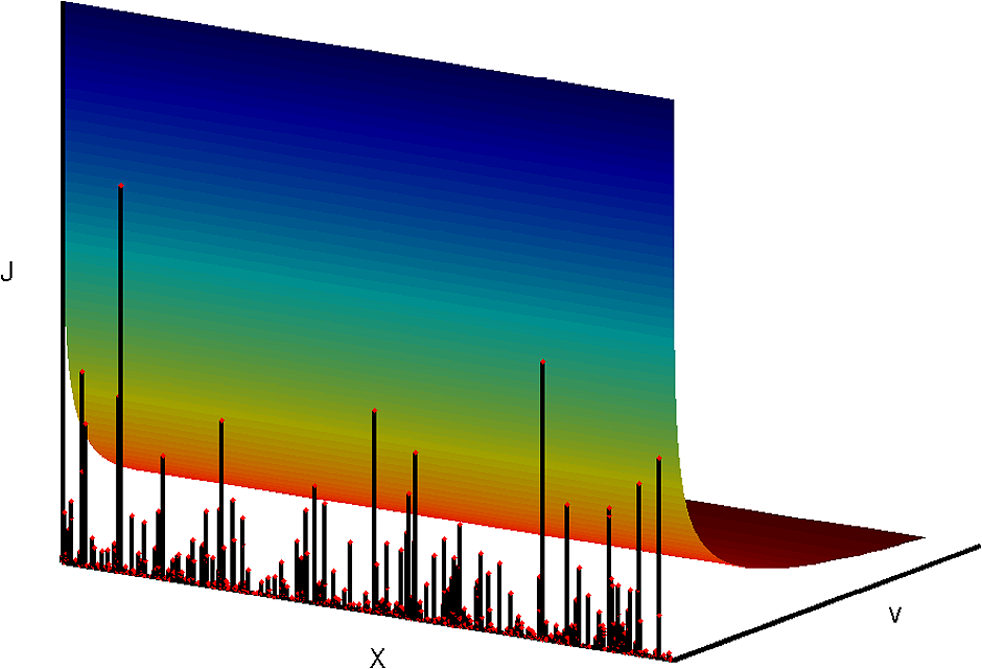
\includegraphics[width=0.6\linewidth]{CRM.png} 
%     \caption{A draw $\sum_{j \ge 1}{J_j \delta_{X_j}}$ from a \gls{CRM}. Each stick denotes an atom in the \gls{CRM}, with mass given by its height $J_j$ and location given by $X_j$. Behind the \gls{CRM} is the density of its Lévy intensity measure $\nu$. Source: \cite{Favaro:2013fl}.}
%     \label{fig:CRM} 
% \end{figure}

It is required that $\mu$ has almost-surely finite total mass, Equation \ref{eq:levy} with $g(y)=1$ shows that the Lévy measure is required to satisfy the property
$$ \int_{\mathbb{R}^+ \times \mathbb{X}} \left( \  1 - e^{-s} \right) \rho(ds) H_0(dy) = 
\int_{\mathbb{R}^+} \left( \  1 - e^{-s} \right) \rho(ds) < \infty $$
Furthermore, the expected number of random atoms in $\mu$ is obtained by Campbell’s Theorem to be the total mass of the Lévy measure $T = \rho(\mathbb{R}^+)$. In typical applications of Bayesian nonparametrics this is infinite, so we can work with mixture models with infinite number of components. This also guarantees that the total mass is positive almost-surely. 

However, since $T \neq 1$ in general, \glspl{CRM} cannot directly be used as priors for mixture models.
One can normalize a \gls{CRM} by its finite total mass to construct a BNP prior for mixture models.\\

\begin{definition}[Normalised Random Measure] \label{def:NRM}
Let $\mu$ be a homogeneous \gls{CRM}, with Lévy measure $\rho$ and base distribution $H_0$, with almost-surely positive and finite total mass. A \gls{NRM} is an almost-surely discrete random probability measure $P$ on $\mathbb{X}$ obtained by normalising $\mu$
$$ P = \frac{\mu}{T} = \sum_{k \ge 1}{p_k \delta_{X^\star_k}} $$
with $T = \sum_{k \ge 1}{J_k}$ and $p_k = J_k / T$.
Since $\mu$ is homogeneous, the law of $\left(p_k \right)_{k \ge 1}$ is governed by the Lévy measure $\rho$ and the atoms $\left(X^\star_k \right)_{k \ge 1}$ are a sequence of random variables independent of $\left(p_k \right)_{k \ge 1}$, and independent and identically distributed according to $H_0$.
We denote it by $P \sim \text{NRM}(\rho, H_0)$. \\
\end{definition}

Let $\mu \sim \text{CRM}(\rho, H_0)$ with an almost-surely finite and positive total mass $T$, and $P = \mu / T$. Suppose that $T$ is positive and finite almost-surely, and absolutely continuous with respect to Lebesgue measure with density $f_\rho(t)$.
Let $(X_i)_{i \ge 1}$ be a sequence of random variables that, given $P$, are independent and identically distributed according to $P$. Since $\mu$ is almost-surely discrete, there is a positive probability that $X_i = X_j$ for each pair $i \neq j$, i.e. when both are assigned to the same atom in $P$. This induces a partition $\pi$ on $\mathbb{N}$, where $i$ and $j$ are in the same block in $\Pi$ if and only if $X_i = X_j$.

We can thus define a mixture model with an \gls{NRM} acting as a \gls{BNP} prior as following:
\begin{gather*}
\mu \sim \text{CRM}(\rho, \mu_0), \\
P = \frac{\mu}{T}, \\
X_i|P \sim P, \\
Y_i|X_i \sim F(\cdot|X_i), \\
\end{gather*}

An example of \gls{NRM} is the \gls{NGGP}. The GGP Lévy measure is
\begin{equation} \label{eq:GGP}
\rho(dy) = \frac{a}{\Gamma(1 - \sigma)}y^{-\sigma-1}e^{-\tau y} dy,
\end{equation}
where $\tau \in [0,\infty)$, $a \in (0, \infty)$ and $\sigma \in [0, 1)$. The \gls{NGGP} is then obtained, as described above, by normalisation of the GGP. Notable special case of \gls{NGGP} are $\sigma = 0$ where we obtain the \gls{DP}, and $\sigma=0.5$, where we obtain the \gls{IG} process.

%The random partition $\Pi$ is exchangeable, and its exchangeable partition probability function (EPPF) can be deduced from the law of the \gls{NRM}.
%Kingman \cite{CIS-16820} demonstrates that there is a correspondence between the law of ⇧ and that of the random probability measure.

\subsection{Poisson-Kingman random probability measure}
Poisson-Kingman \gls{RPM} were introduced in \cite{pitman2003pkp} as a generalisation of homogeneous NRMs. \\

\begin{definition}[Poisson-Kingman Random Probability Measure] \label{def:PKRPM}
Let $\mu \sim \text{CRM}(\rho, H_0)$ and let $T = \mu(\mathbb{X})$ be finite, positive almost-surely, and absolutely continuous with respect to Lebesgue measure. For any $t \in \mathbb{R}^+$, let us consider the conditional distribution of $\mu/t$ given that the total mass $T \in dt$. This distribution is denoted by $\text{PK}(\rho, \delta_t , H_0)$, were $\delta_t$ denotes the Dirac delta function. Poisson-Kingman \glspl{RPM} form a class of \glspl{RPM} whose distributions are obtained by mixing $\text{PK}(\rho, \delta_t , H_0)$, over $t$, with respect to some distribution  $\gamma$ on the positive real line. Specifically, a Poisson-Kingman \gls{RPM} has the hierarchical representation
$$T \sim \gamma, $$
\vspace{-2em}
\begin{gather} \label{eq:PK}
P|T=t \sim \text{PK}(\rho, \delta_t, H_0),
\end{gather}
The \gls{RPM} $P$ is referred to as the Poisson-Kingman \gls{RPM} with Lévy measure $\rho$, base distribution $H_0$ and mixing distribution $\gamma$. The distribution of $P$ is denoted by $\text{PK}(\rho, \gamma , H_0)$. If the density for the total mass equals the density obtained from its Lévy measure $f_\rho$, i.e. $\gamma(dt) = f_\rho(t) dt$, then the distribution $\text{PK}(\rho, f_\rho , H_0)$, coincides with $\text{NRM} (\rho, H_0)$.
\end{definition}

Since $\mu$ is homogeneous, the atoms $\left(X^\star_k \right)_{k \ge 1}$ of $P$ are independent of their masses $\left(p_k \right)_{k \ge 1}$. They form a sequence of independent random variables identically distributed according to $h_0$. Finally, the masses of $P$ have distribution governed by the Lévy measure $\rho$ and the distribution $\gamma$.

Same as for \glspl{NRM}, Poisson-Kingman \glspl{RPM} can be used as \gls{BNP} prior for mixture models. The associated hierarchical model is the following:
\begin{gather*}
T \sim \gamma, \\
P|T=t \sim \text{PK}(\rho, \delta_t, H_0), \\
X_i|P \sim P, \\
Y_i|X_i \sim F(\cdot|X_i),
\end{gather*}

% \begin{figure}[h!]
% \centering
%     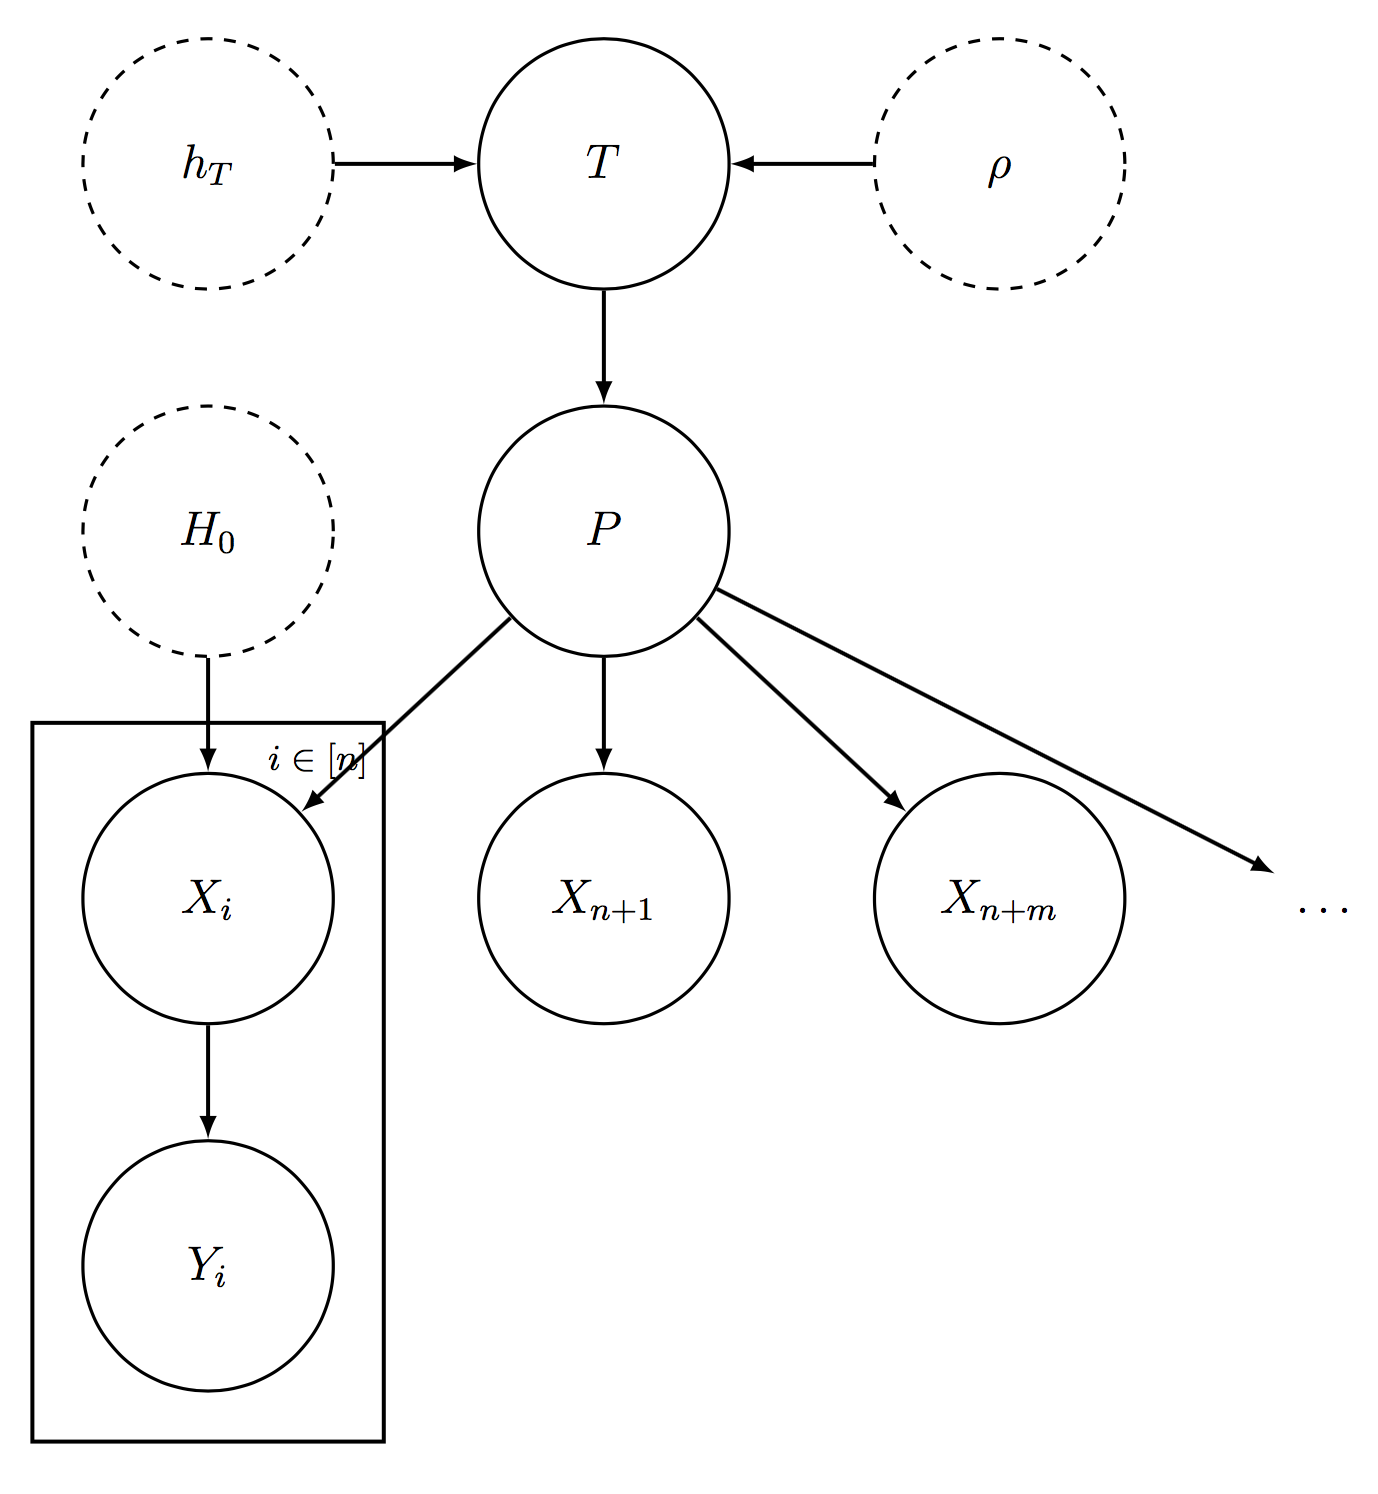
\includegraphics[width=0.5\linewidth]{graph_model_intractable.png} 
%     \caption{\gls{PKP} intractable graphical model: the latent variables are countably infinitely many which makes the model computationally intractable. Source: \cite{LomeliThesis}.} 
%     \label{fig:graph_model_intractable} 
% \end{figure}
Figure \ref{fig:graph_model_intractable} represents the associated graphical model.

\paragraph{$\sigma$-Stable Poisson-Kingman \glspl{RPM}}
One famous class of Poisson-Kingman \gls{RPM} is the class $\sigma$-Stable Poisson-Kingman \glspl{RPM} which encompasses most of the popular discrete \glspl{RPM} used in Bayesian nonparametrics, for instance, the Pitman-Yor process and the normalised generalised Gamma process.
For any $\sigma \in (0,1)$ the density function of a positive  $\sigma-$Stable random variable is
$f_\sigma(t) = \frac{1}{\pi}\sum_{j=0}^\infty \frac{(-1)^{j+1}}{j!}\sin(\pi\sigma j)\frac{\Gamma(\sigma j+1)}{t^{\sigma j+1}}$. A $\sigma$-Stable Poisson-Kingman \gls{RPM} is a Poisson-Kingman \gls{RPM} with Lévy measure given by
\begin{equation} \label{eq:sigma_stable_PK}
\rho(dy) := \rho_\sigma(dy) = \frac{a}{\Gamma(1 - \sigma)}y^{-\sigma-1} dy,
\end{equation}
and base distribution $H_0$.
The mixing distribution for the total mass $T$ takes the following 
$\gamma(dt) \propto h(t) f_\sigma(t) dt$, for any non-negative measurable function $h$ such that
$\int_0^\infty{h(t)f_\sigma(t) dt} < \infty$.
Accordingly, $\sigma$-Stable Poisson-Kingman \glspl{RPM} form a class of discrete \glspl{RPM} indexed by the parameters $(\rho, h)$. The Dirichlet process can be recovered as a limiting case, if $\sigma \rightarrow 0$, for some choices of $h$. The following examples of $\sigma$-Stable Poisson-Kingman \glspl{RPM}  are obtained by specifying the tilting function $h$. See \cite{LomeliThesis} for more examples and more details on those.

\begin{itemize}
\item \acrfull{NS}: $h(t) = 1$
\item \acrfull{NGGP} : $h(t) = \exp\{\tau - \tau^{1/\sigma}t \}$, for any $\tau > 0$
\item \acrfull{PY}: $h(t) = \frac{\Gamma(\theta + 1)}{\Gamma(\theta / \sigma + 1)}t^{-\theta}$ with $\theta \ge -\sigma$
\item \acrfull{GT}: $h(t) = t^{-\theta} \exp\{-\eta t\}$ for any $\eta > 0$ or $\eta=0$ and $\theta>-\sigma$
\item \acrfull{pgc}: $h(t) = \int_{\mathbb{R}^+} \exp\{\tau - \tau^{1/\sigma}t \} F(d\tau)$ \\
\end{itemize}

\textcolor{red}{BETTER TRANSITION ?}
The conditioning operation from the generative process from Equation \ref{eq:PK} is not well defined a priori but the following proposition from \cite{Perman:1992ke} helps to bypass this difficulty. It also states an interesting Markovian property of the surplus masses, which will be of used to describe a \gls{PK} generative process. \\

\begin{proposition}[Perman et al. \cite{Perman:1992ke}] \label{prop:perman}
The sequence of surplus masses $\left(T_k \right)_{k \ge 0}$ forms a Markov chain, where $T_k := T - \sum_{l=1}^k J_l$ , with initial distribution and transition kernels given as follows
\begin{equation*}
\begin{aligned}
\mathbb{P}_{\rho,H_0}(T_0 \in dt_0) &= f_\rho(t_0)dt_0 \\
\mathbb{P}_{\rho,H_0}(T_k \in dt_k|T_0 \in dt_0,\dots, T_{k-1} \in dt_{k-1}) &=  \mathbb{P}_{\rho,H_0}(T_{k-1} \in dt_{k-1})\\
&= \frac{(t_k-t_{k-1})\rho(d(t_k-t_{k-1}))}{t_{k-1}} \frac{f_\rho(t_{k-1})}{f_\rho(t_{k-1})} \\
\end{aligned}
\end{equation*}
\end{proposition}


A sec
ond object induced by a Poisson-Kingman \gls{RPM} is a size-biased permutation of its atoms. Specifically, order the blocks in the partition $\Pi$ (induced by the \gls{RPM}) by increasing order of the least element in each block, and for each $l \in \mathbb{N}$ let $Z_l$ be the least element of the $l$-th block. $Z_l$ is the index among $(X_i)_{i \ge 1}$ of the first appearance of the $l$-th unique value in the sequence.
Let $\tilde{J}_l = \mu(\{X_{Z_l}\})$ be the mass of the corresponding atom in $\mu$. Then $(\tilde{J}_l)_{l\ge 1}$ is a size-biased permutation of the masses of atoms in $\mu$, with larger masses tending to appear earlier in the sequence. It is easy to see that $\sum_{l \ge 1}{\tilde{J}_l} = T$, and that the sequence can be understood as a stick-breaking construction: start with a stick of length $T_0 = T$; break off the first piece of length $\tilde{J}_1$; the surplus length of stick is $T_1 = T - \tilde{J}_1$; then
the second piece with length $\tilde{J}_2$ is broken off, etc.

Proposition \ref{prop:perman} \cite{Perman:1992ke} states that the sequence of surplus masses $(T_l)_{l \ge 1}$ forms a Markov chain and gives the corresponding initial distribution and transition kernels. The density of $T$ is denoted by $\gamma(t) \propto h(t) f_\rho(t)$. The \gls{PK} generative process for the sequence $(X_i)_{i \ge 1}$ goes as follows, where parts of the \gls{PK} random measure $\mu$ are simulated as required.

\begin{enumerate}[label=(\roman*)]
    \item Draw from the total mass from its distribution $\mathbb{P}_{\rho,H_0}(T \in dt) \propto h(t) f_\rho(t)$.
    \item The first draw $X_1$ from $\mu/T$ is a size-biased pick from the masses of $\mu$. The actual
value of $X_1$ is simply $X_1^\star \sim H_0$, while the mass of the corresponding atom in $\mu$ is
$\tilde{J}_1$, with conditional distribution given by
$$ \mathbb{P}_{\rho,H_0}(\tilde{J}_1 \in ds_1 | T \in dt) = \frac{s_1}{t}\rho(ds_1)\frac{f_\rho(t - s_1)}{f_\rho(t)} $$
The leftover mass is $T_1 = T - \tilde{J}_1$.
    \item For subsequent draws $i \ge 2:$
    \begin{itemize}
        \item Let $k$ be the current number of distinct values among $X_1,\dots,X_{i-1}$, and let
$X_1^\star,\dots,X_{k}^\star$ be the unique values, i.e., atoms in $\mu$. The masses of these first
$k$ atoms are denoted by $\tilde{J}_{1},\dots,\tilde{J}_{k}$ and the leftover mass is $T_k = T - \sum_{l=1}^k{\tilde{J}_{l}}$.
        \item For each $l \le k$, with probability $\tilde{J}_l / T$, we set $X_i = X_l^\star$.
        \item With probability $T_k / T$, $X_i$, takes on the value of an atom in $\mu$ besides the first $k$ atoms. The actual value $X_{k+1}^\star$ is drawn from $H_0$, while its mass is drawn from
        $$ \mathbb{P}_{\rho,H_0}(\tilde{J}_{k+1} \in ds_{k+1} | T \in dt_k) = \frac{s_{k+1}}{t_k}\rho(ds_{k+1})\frac{f_\rho(t_k - s_{k+1})}{f_\rho(t_k)} $$
        The leftover mass is again $T_{k+1} = T_k - \tilde{J}_{k+1}$.
    \end{itemize}
\end{enumerate}

By multiplying the above infinitesimal probabilities one obtains the joint distribution of the random elements $T$, $\Pi$, $(\tilde{J}_i)_{i \ge 1}$ and $(X_i^\star)_{i \ge 1}$.
\textcolor{red}{write joint distribution ?}

\section{MCMC Inference}
Constructing \gls{MCMC} schemes for models with one or more Bayesian nonparametric components is an active research area since dealing with the infinite dimensional component $P$ forbids the direct use of standard simulation-based methods. These methods usually require a finite-dimensional representation. The general idea for designing inference schemes is to find finite dimensional representations to be able to store the model in a computer with finite capacity.

There are two main sampling approaches to facilitate simulation in the case of Bayesian nonparametric models: random truncation and marginalisation. These two schemes are known in the literature as conditional and marginal, but hybrid samplers between these two also exist. Each sampler rely on a tailored, thus different, representation of the underlying process. Yet, these samplers are all instances of Gibbs sampler.

\subsection{Marginal Samplers}
% \begin{figure}[h!]
% \centering
%     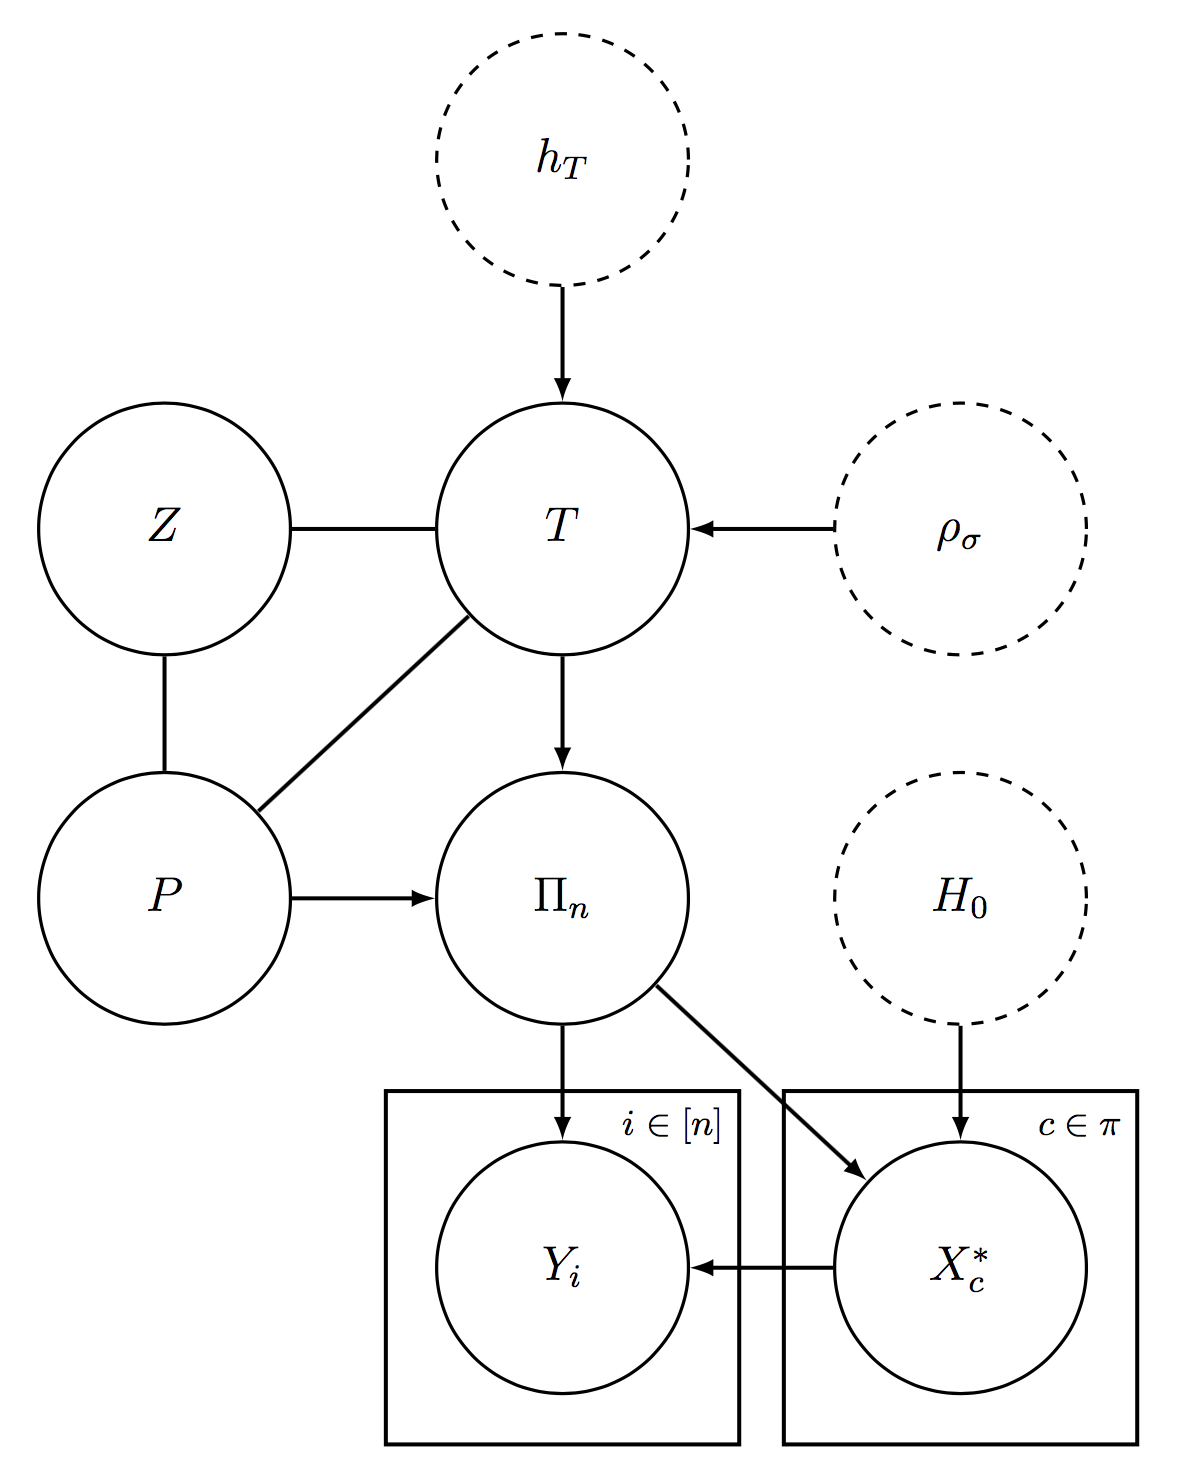
\includegraphics[width=0.5\linewidth]{graph_model_marginal.png} 
%     \caption{Marginal sampler’s graphical model. Each node represents a variable used in the augmented representation for the joint distribution. The nodes with dashed lines represent the algorithmic inputs. Source: Maria Lomeli's thesis} 
%     \label{fig:graph_model_marginal} 
% \end{figure}

Marginal samplers bypass the need to represent the infinite-dimensional component by marginalising it out. These schemes have lower storage requirements than conditional samplers because they only store the induced partition, but could potentially have worse mixing properties.

With a conjugate model ($H_0$ and $F$ are conjugate), both the \gls{RPM} $P$ and the cluster parameters $\{X_c^\star: c \in \pi \}$ can be marginalised out efficiently. Yet, for a more generic nonconjugate marginalized sampler, the cluster parameters cannot be easily marginalised out and are thus included into the state of the \gls{MCMC} algorithm. This yields the difficulty of the introduction of new clusters (along with their parameters) when Gibbs sampling the cluster assignments.

To tackle this issue, \cite{Neal:2000hb} conceptualizes the update in terms of an augmented state with additional temporarily existing variables, in a way that the marginal distribution of the permanent variables once the temporary ones are integrated out is still the appropriate posterior distribution.
To do so, the state space is augmented as well to include both existing clusters and new empty clusters $[M] = \{1, \dots , M\}$, which parameters are independent of the existing ones and independent and identically distributed according to $H_0$.
\cite{Favaro:2013fl} extends this idea originally developed for \gls{DP} mixtures, for all \gls{NRM} mixture models.

For instance, if the $\sigma$-Stable Poisson-Kingman subclass is picked, then it is possible to obtain a tractable representation, given by Figure \ref{fig:graph_model_intractable}, in terms of some random variables and the partition induced by the \gls{RPM}.
This representation is based on an augmented version of its corresponding exchangeable partition probability function.

\subsection{Conditional Samplers}
% \begin{figure}[h!]
% \centering
%     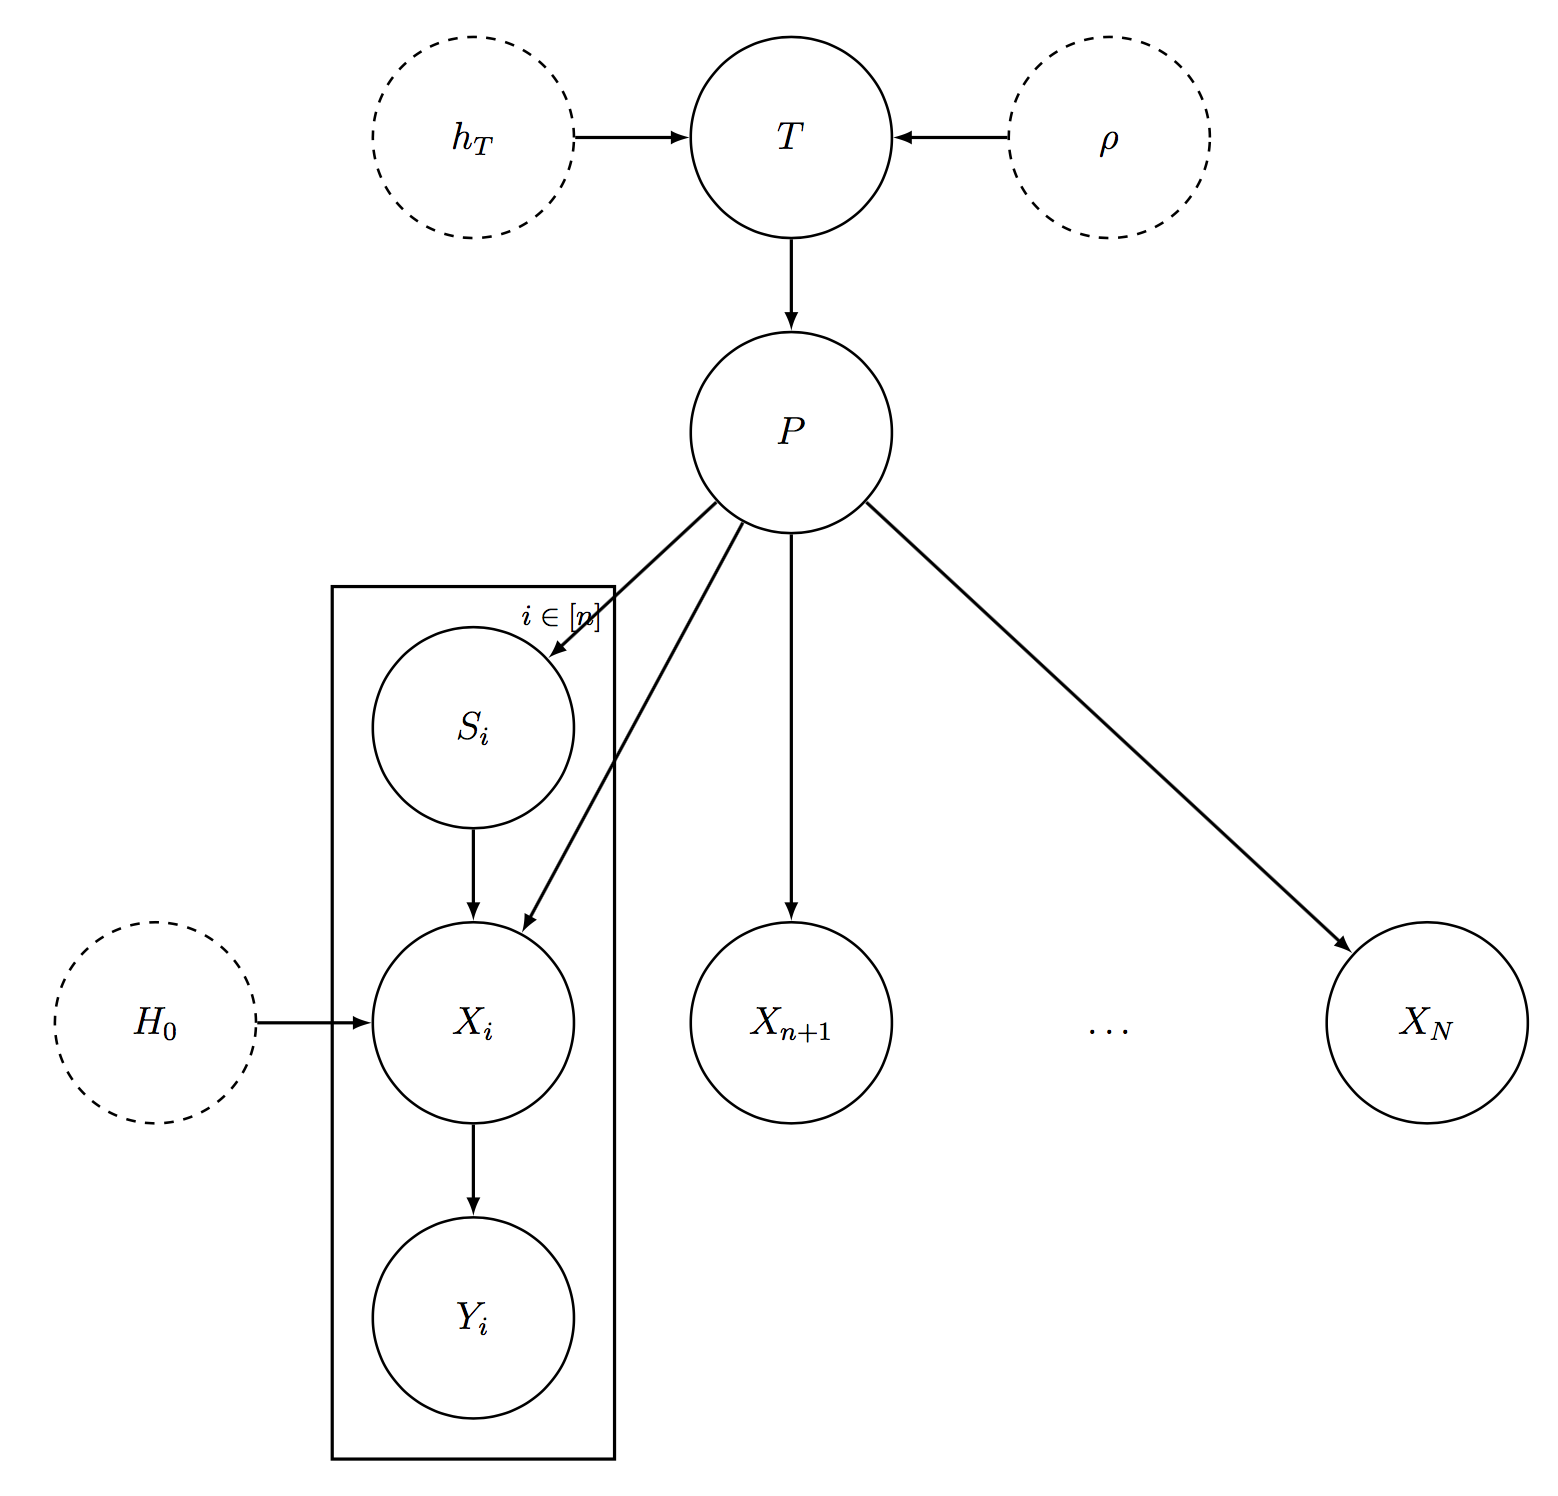
\includegraphics[width=0.5\linewidth]{graph_model_conditional.png} 
%     \caption{Conditional sampler’s graphical model. Each node represents a variable used in the augmented representation for the joint distribution. The latent variables represent the number of occupied and unoccupied components. Source: \cite{LomeliThesis}.} 
%     \label{fig:graph_model_conditional} 
% \end{figure}

Conditional samplers replace the infinite-dimensional prior by a finite-dimensional representation chosen according to a truncation level. Since these samplers do not integrate out the infinite-dimensional component, their output provides a more comprehensive representation of the random probability measure.
Figure \ref{fig:graph_model_conditional} shows such representation or the $\sigma$-Stable Poisson–Kingman
family for the conditional slice \gls{MCMC} sampler \cite{FavaroWalker2012}.

The truncation level needs to be randomised to have an exact \gls{MCMC} scheme. A slice sampling step \cite{neal2003} within the Gibbs sampler is used in \cite{Favaro:2013fl} so as to get an efficient sampler.
It allows to represent a finite but random number of stick-breaking weights. These weights correspond to the ones that fall above the slice variables, sampled at every iteration. Then, the cluster assignment variable for each observation is chosen from a categorical distribution, where the number of categories given by the number of represented sticks. For this reason, both the number of occupied and empty clusters is stored at every iteration. These numbers could be potentially large.

The stick-breaking weights can be sampled either via a stick-breaking representation of the measure, or via thinning \cite{Favaro:2013fl}. Unfortunately, only few models have a tractable stick-breaking representation, such as the \gls{DP}, the \gls{PY} or a sub-class of $\sigma$-stable Poisson-Kingman models \cite{Favaro:2014bo}.


\subsection{Hybrid Samplers}
% \begin{figure}[h!]
% \centering
%     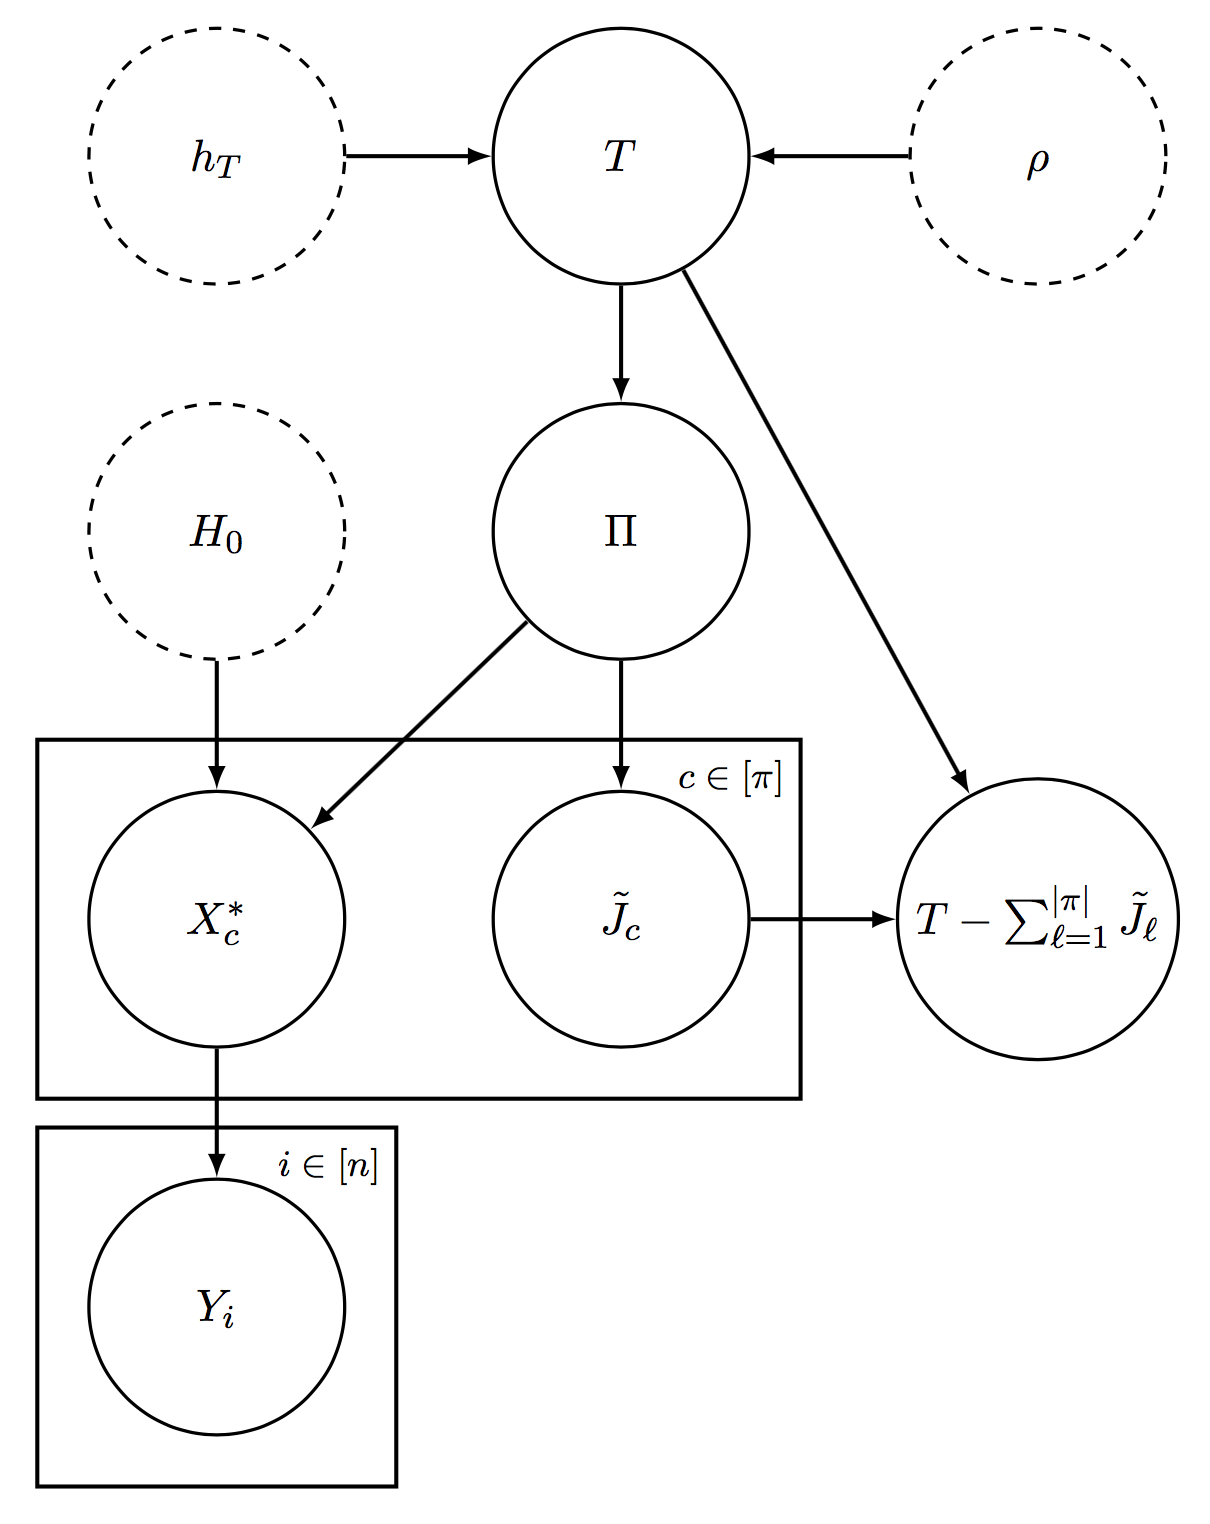
\includegraphics[width=0.5\linewidth]{graph_model_hybrid.png} 
%     \caption{PK hybrid sampler’s graphical model. Each node represents a variable used in the augmented representation for the joint distribution. The nodes with dashed lines represent the algorithmic inputs. Source: \cite{LomeliThesis}.} 
%     \label{fig:graph_model_hybrid} 
% \end{figure}

A third hybrid \gls{MCMC} scheme has been developed \cite{Lomeli:2015vd}, and combines the main strengths of both conditional and marginal \gls{MCMC} samplers.

This hybrid scheme makes use of a representation of the model where only the size-biased weights associated to occupied clusters are needed to be explicitly represented along with a surplus mass term, associated to the rest of the empty clusters.
Figure \ref{fig:graph_model_hybrid} shows this tractable and compact representation for a Poisson-Kingman mixture model is based.
The cluster reassignment step can be seen as a retrospective sampling scheme: we explicitly represent and update the weights associated to occupied clusters and create a new size-biased weight only when a new cluster appears. %To make this possible, we use the induced partition.

This scheme has less memory requirements since it only represents the size-biased weights associated to occupied clusters as opposed to conditional samplers which represent both empty and occupied clusters. Also, since it does not integrate out all of the size-biased weights, we obtain a more comprehensive representation of the \gls{RPM}.

\subsection{Sequential Monte Carlo}
Recently, various \gls{SMC} schemes (see Section \ref{SMC} for more details on \gls{SMC}) for Bayesian nonparametric models have been proposed.
\cite{Fearnhead:2004gi} and \cite{Wood:2008hx} propose an \gls{SMC} scheme for Dirichlet process mixture models and \cite{Griffin:2017cz} for \gls{NRM} mixture models.
These articles cast the marginal and conditional representations presented previously in a particle algorithm's setting.

\section{Variational inference} \label{BNP_VI}
To my knowledge, the first article tackling inference in a \gls{BNP} setting is \cite{Blei:2006fo}, where
a truncated proposal is introduced to approximate a Dirichlet Process Mixture model.

\textit{Truncation-free} \acrlong{VI} methods have also been introduced \cite{Blei:2012uu}. These methods adapts model complexity on the fly by lazily representing clusters assignments. Yet, the sticks proportions and mixture components are marginalize out to obtain a closed form distribution for the mixture assignment hidden variables $z_i$. This marginalization is unfortunately only tractable for few models, such as the Dirichlet Process and the Pitman-Yor process.
